\documentclass[12pt]{article}
\usepackage{amssymb}
\usepackage{geometry}
\usepackage{graphicx}
\usepackage{hyperref}
\usepackage{wrapfig}
\usepackage{amsmath}
\usepackage{lipsum}
\usepackage{caption}
\usepackage{ulem}
\usepackage{xcolor}
\usepackage{tikz}
\usetikzlibrary{arrows.meta, positioning, shapes}

\usepackage{sectsty}
\sectionfont{\color{sectionColor}}       % Color for \section
\subsectionfont{\color{subsectionColor}}


\definecolor{titleColor}{HTML}{800000}        % Maroon
\definecolor{sectionColor}{HTML}{4682B4}      % SteelBlue
\definecolor{textHighlight}{HTML}{DAA520}     % Goldenrod
\definecolor{backgroundColor}{HTML}{F0F8FF}   % AliceBlue
\definecolor{emphasisColor}{HTML}{228B22}     % ForestGreen
\definecolor{subsectionColor}{HTML}{6A5ACD}   % SlateBlue


\title{\textcolor{titleColor}{\textbf{\Huge \textbf{Heart-hub a web application}}}}

\author{B. M. Osman\thanks{Al Nahada University, Cairo \\ \texttt{babikerosman@yahoo.com}}}
\date{\today}
\begin{document}
\maketitle



\begin{document}

The URL 
\url{https://hearthub-bjyb3bzoe-babikerosmans-projects.vercel.app/dashboard.html} 
points to a deployment of \textbf{HeartHub}, a web application hosted on Vercel.

HeartHub is an open-source Python toolkit by GitHub user 
\href{https://github.com/babikerosman468/Hearthub}{babikerosman468}, 
focusing on heart-based data science, coherent consciousness research, and community resilience modeling.

The GitHub repository provides backend tools and documentation, but does not include a detailed frontend dashboard. 
The deployed URL appears to serve as a custom frontend interface. 
Without access to the source code or further documentation, a detailed description of its functionalities is limited.

For further exploration or contribution, the project repository can be accessed at 
\href{https://github.com/babikerosman468/Hearthub}{GitHub}.


\begin{wrapfigure}{r}{0.35\textwidth}                       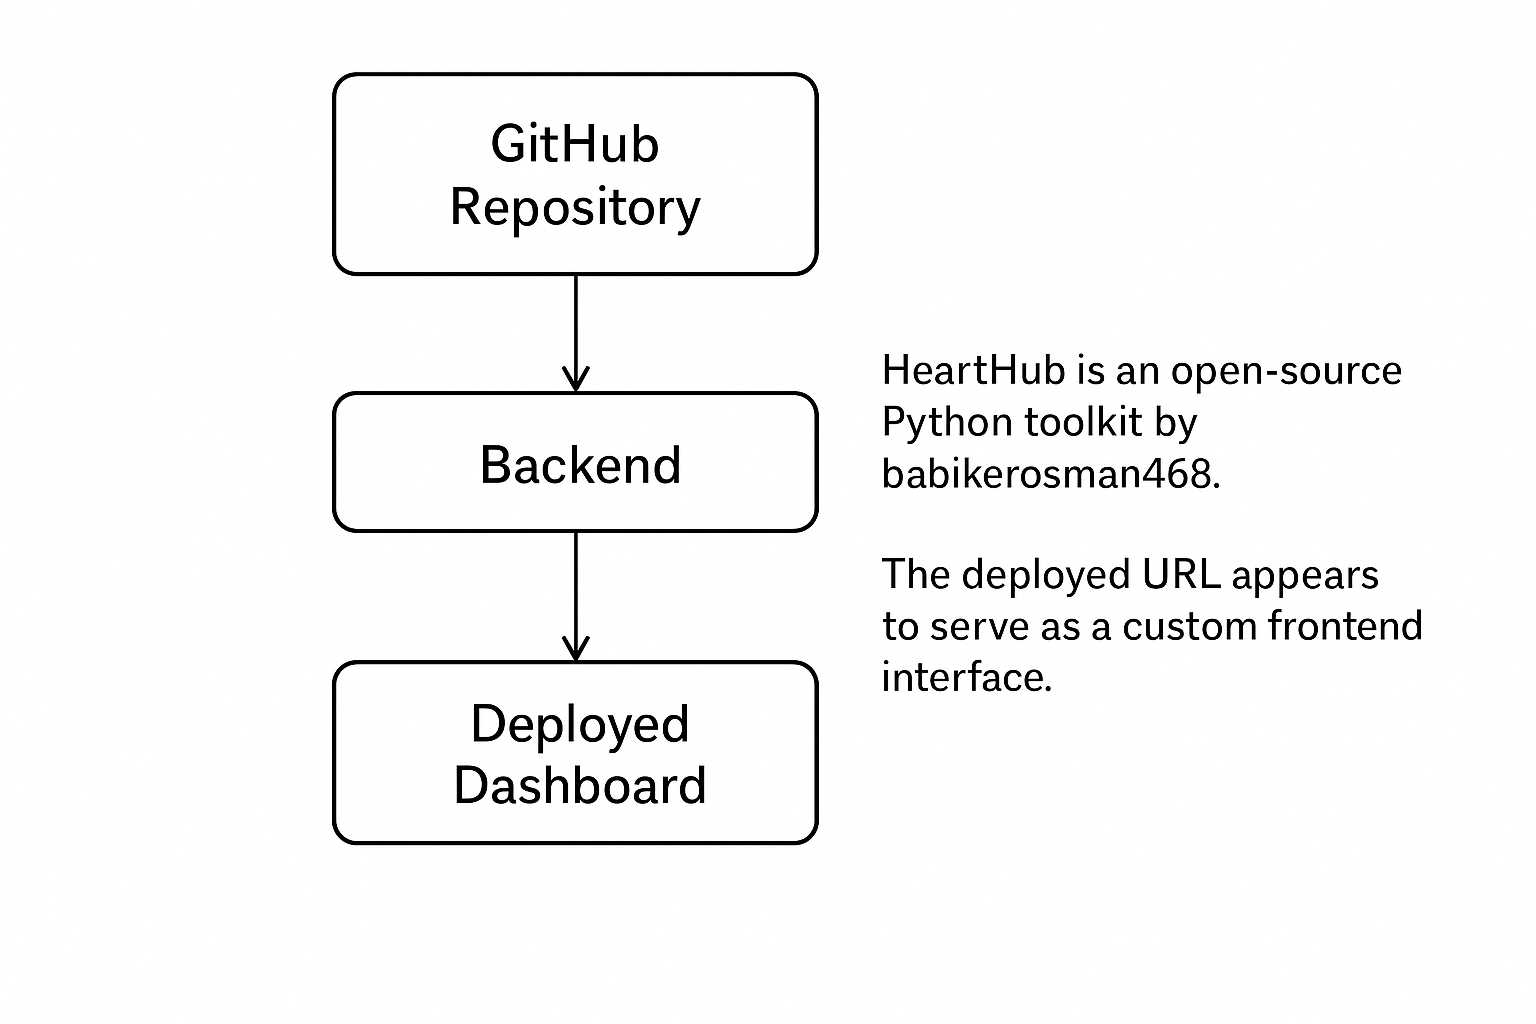
\includegraphics[width=0.35\textwidth]{6.png}
\caption{ \textbf{Hearthub} }      \end{wrapfigure}


\end{document}

